\chapter{Introduction}
\label{sec:introduction}

Twenty years ago, Lieberman described debugging as "the dirty little secret of computer science".
He argued that the huge economic cost created by software bugs, resulting from the efforts to locate and fix bugs and the damages caused by bugs  not found in time, was not adequately matched by efforts to provide and establish better debugging tools and practices.
Lieberman called this the "Debugging Scandal"~\cite{lieberman_97_the_debugging_scandal}.
Twenty years later, the situation has barely improved.

The amount of software that is involved in almost every aspect of our modern life is steadily increasing.
In many fields, innovation is largely driven by software~\cite{evans_08_invisible_engines_how_software, gorschek_10_a_lightweight_innovation_process}.
With the rise of cloud computing and devices becoming smarter and smarter, this trend will not stop in the near future.

It has long been recognized that there is no such thing as a bug-free program~\cite{schwartz_71_an_overview_of_bugs}.
Errors affect the operation of all professional and commercial software products, from web-browser~\cite{li_06_have_things_changed_now}, over enterprise applications~\cite{turhan_09_data_mining_source_code, sahoo_10_an_empirical_study}, to operating systems~\cite{guo_10_characterizing_and_predicting_which}\todo{.}. % check sources

In 2002, the yearly economic cost of software errors was estimated to be above 60 billion dollars in the United States alone~\cite{tassey_02_the_economic_impacts}. 
Additional billions of damage are created by failing software projects, where bugs are at least part of the problem~\cite{charette_05_why_software_fails}.

Studies found that developers spend between 25\% and 60\% of their time on software bugs, debugging, and related activities~\cite{ballou_08_improving_software_quality, hailpern_02_software_debugging_testing, beizer_03_software_testing_techniques}.
Considering the total cost created by bugs in software, we would expect companies to encourage software developers to improve their debugging skills (e.g., through trainings) and to use modern debugging techniques.
However, 72\% of software companies report their debugging practices to be problematic~\cite{ballou_08_improving_software_quality}.

%\cite{beck_03_testdriven_development_by_example, williams_03_testdriven_development_as}

\section{35 Years of Debugging Research are Barely Used in Practice}

Ever since Grace Hopper famously taped into a log book a moth that was causing computer errors, thereby bringing the term "debugging" into software engineering, a lot of work has been done to help developers to locate bugs in their software.

Back in the 1940s and 50s, debugging had to be done statically.
In the best case, a post-mortem data dump from the moment of the failure was available.
Because modifying and re-running a program was expensive and time-consuming, bugs could only be located by manually analyzing the code.

In the 1960s, the invention of operating systems with time-sharing capabilities allowed developers to use the "edit -- compile -- run" loop.
By experimenting with changes to the source code, it was much easier to get an understanding of the problem.
Furthermore, interactive terminals allowed developers to insert trace statements into the code, which could report internal states and program flow.
This practice is also known as "printf"-debugging and remains popular to this day~\cite{perscheid_17_studying_the_advancement}.

At the same time, with the "Dynamic Debugging Technique" (DDT) and later EXDAMS the first tools were developed to facilitate stepwise executions of programs and to let developers examine program state~\cite{balzer_69_exdams_extendable_debugging}\todo{source: ddt}.
In the 1970s, debuggers moved to the command line and the introduction of the breakpoint allowed developers to pause the execution at predefined points.
In 1975, the first debugger (for COBOL) integrated compiler information to translate identifiers from the source code into memory addresses and vice versa, alleviating developers from manually performing this task.
Such symbolic debuggers are, when available, widely used today; unfortunately, as we will see, they are also the most recent innovation that found wide adoption in pracitce~\cite{perscheid_17_studying_the_advancement}.

In 1982, Weiser introduced the concept of slices, subsets of statements in a program that influence each other~\cite{weiser_81_program_slicing}. 
He showed that slices are a useful abstraction for programmers who think about code~\cite{weiser_82_programmers_use_slices_when}.
Later this concept was extended to consider runtime data for higher precision~\cite{agrawal_90_dynamic_program_slicing, korel_90_dynamic_slicing_of_computer}.

Early on it was noted that given the way debuggers follow infection chains, by trying to find the source for an incorrect value, it would be helpful to go backwards through a program execution.
Debuggers that used snapshots~\cite{feldman_88_igor_a_system} or reverse execution~\cite{lieberman_95_zstep_95_a_reversible} were developed in the 1990s.
In 2003, Lewis introduced the concept of "omniscient debugging", a debugger that can not only run forwards and backwards in time, but has instantaneous access to every state in past, present, and future~\cite{lewis_03_debugging_backwards_in_time}.

Although both slicing and omniscient debugging can answer many questions developers have while debugging that regular debuggers can't answer~\cite{ko_07_information_needs_in_collocated, storey_97_how_do_program_understanding, sillito_06_questions_programmers_ask}, neither technique is widely used, or even widely known, today~\cite{perscheid_17_studying_the_advancement}.

\begin{figure*}[th]
\centering
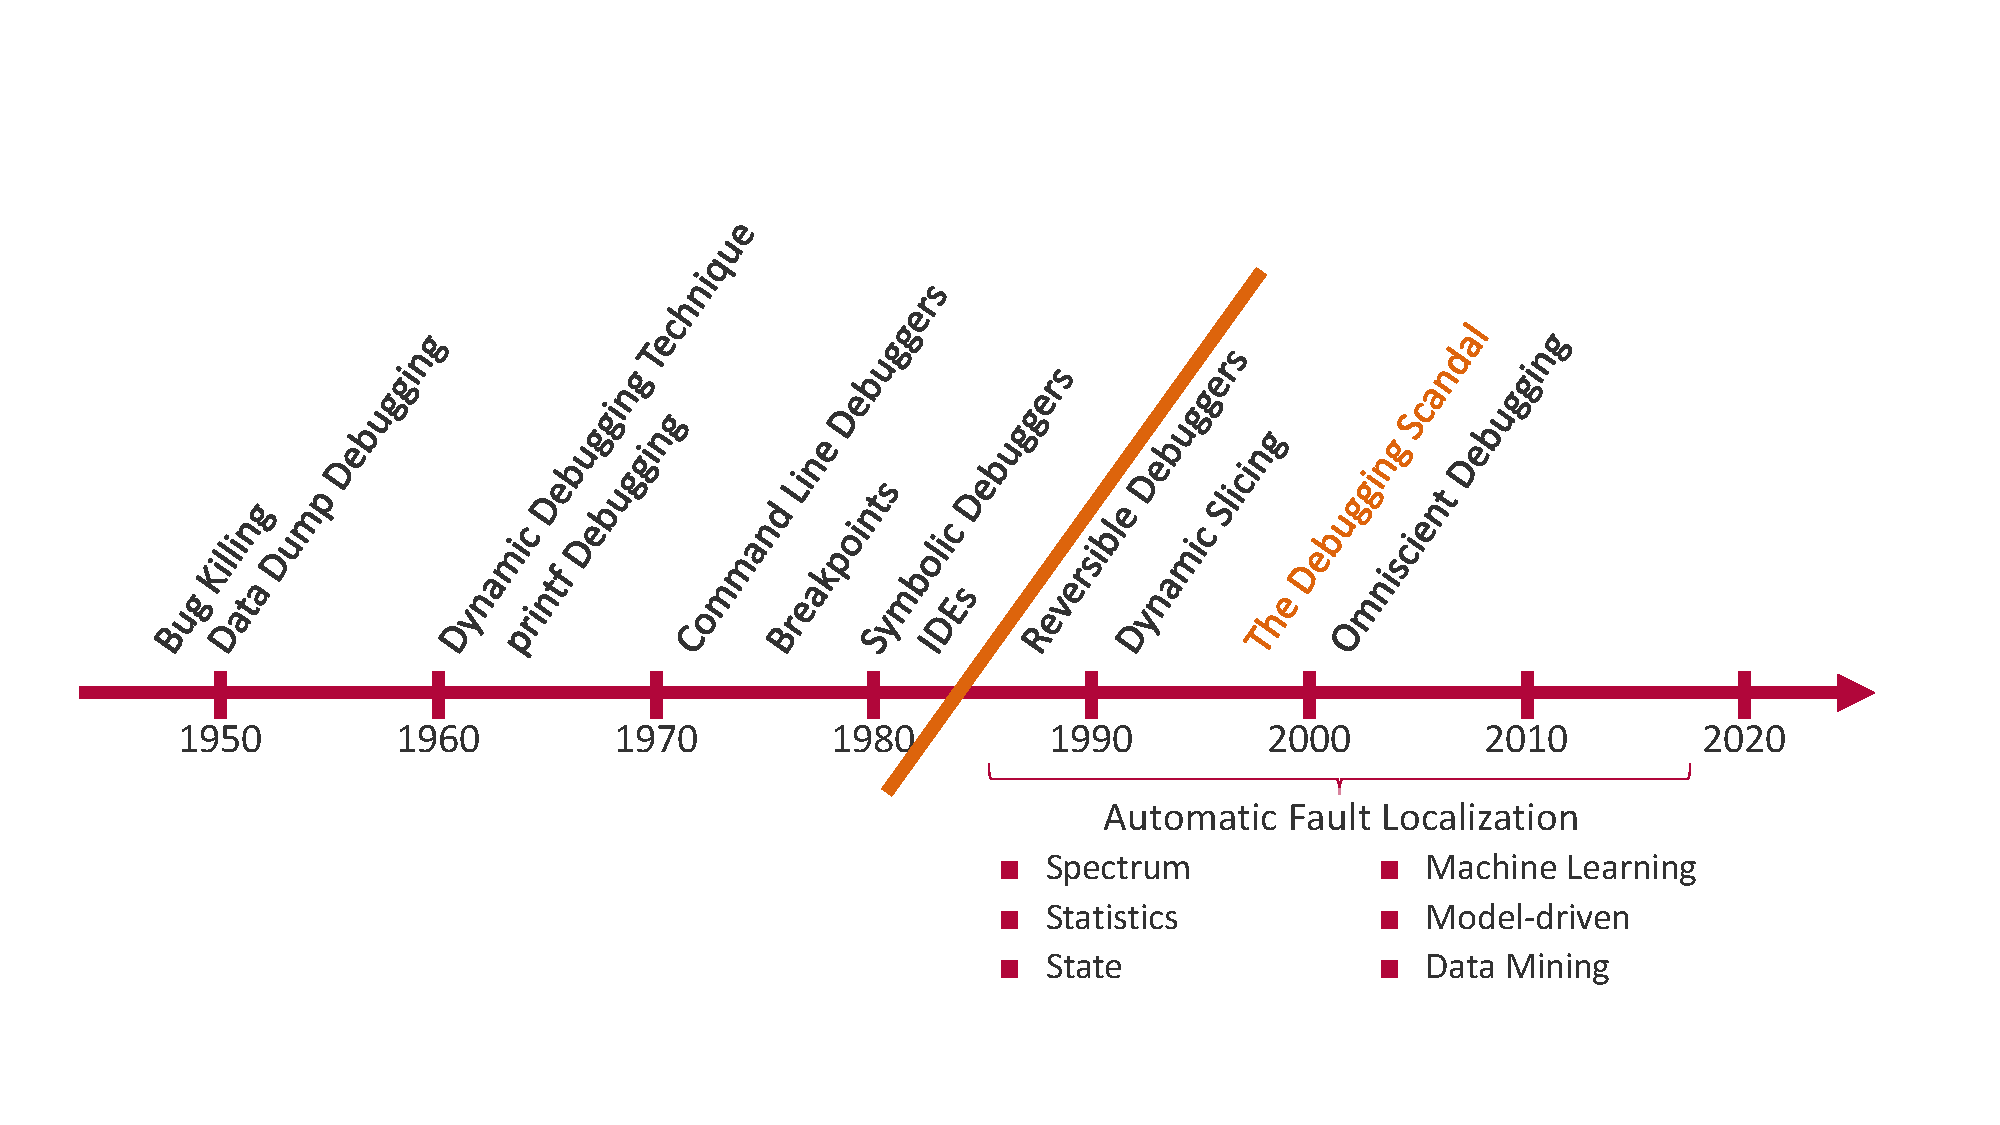
\includegraphics[width=\linewidth]{img/debugging-timeline}
\caption{A brief timeline of debugging history and the gap between research and practice.}
\label{fig:debugging-timeline}
\end{figure*}

\begin{figure*}[th]
\centering
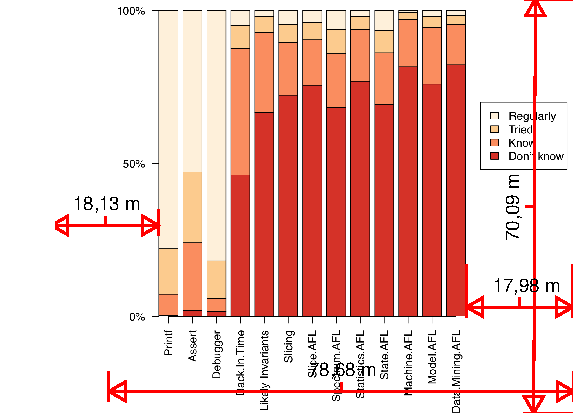
\includegraphics[width=.6\linewidth]{img/tool-usage}
\caption{Answers to "Which debugging tools do you know?"~\cite{perscheid_17_studying_the_advancement}.}
\label{fig:tool-usage}
\end{figure*}

\section{Are There Too Many Debugging Tools?}

What we find today is a large number of debugging tools, techniques, and prototypes that are very good at what they do, but not very accessible to developers.

In interviews we have learned that many developers are not even aware that advanced debugging techniques (i.e., anything beyond symbolic debugging) exist and may even be available for the programming languages they use.
If developers know of an advanced debugging tool, they often cite a lack of documentation as the main reason for not using it.
While locating a software fault, developers don't want to divert attention to learning a new tool.


On top of accessibility concerns, new requirements have emerged for debugging tools:
% Context
Complex systems often consist of multiple inter-operating components written in different programming languages and running in different environments.
Many enterprise applications, for example, follow a three-tier architecture.

A database layer handles persistence and data-intensive computations.
On top, the application layer implements most of the business process logic and acts as a gateway to the client.
In the client, the user interface layer provides a rich user experience and sends requests to the application back-end to trigger actions and obtain data.

Because of the heterogeneous technologies, each layer typically comes with its own tool set and no tool can be used to work on all layers at once.

% Problem
Bugs can occur in any layer but often only manifest themselves as failures in the user interface.
Thus, developers first have to guess in which layer the error originated before choosing the appropriate debugging tool for that layer.
If the guess turns out to be wrong, developers have to switch tools and context before continuing the bug hunt.
Locating bugs in the interaction between two layers becomes even more difficult, as developers may have to switch tools several times to understand the fault.

To efficiently debug a multi-tier application, developers would need a single debugger that is not only capable of debugging each layer but also aware of the interaction between layers at a meaningful level of abstraction.
Furthermore, to help developers handle the complexity and size of an enterprise application, the debugger should provide analysis features that integrate in the debugging process, instead of interrupting it.

% Significance ?
% Solution
\section{Our Approach} %(Research Questions \& Contributions)

The overarching motivation of this work is to improve debugging to reduce the time and effort needed to locate faults in enterprise applications.
This challenge will be approached from two directions.
First, recent debugging innovations need to be made more available in practice.
It is not enough to simply make more features available in debugging tools, the features need to be conveniently accessible and the cost of learning a new feature must not be too high at any point in time.
Second, debugging tools need to move along with recent technology trends.
Developers need better support debugging applications that handle large amounts of data and are composed of sub-systems with heterogeneous technology stacks.
From this, three research questions followed.

%\newcommand{\RQ}[1]{\paragraph{\emph{#1}}}
\newcommand{\RQ}[1]{\subsection*{#1}}
% mtiier verbessern ; verfolgen

\RQ{Research Question 1: How can debuggers help developers to navigate a program execution when following a long infection chain?}

When developers debug a program, they are typically not just "browsing" the execution, but rather searching for something specific.
While omniscient debuggers make it easier to effectively navigate a program execution, they offer no specific help for tracking down relevant code locations.
The debugger's vast knowledge about the execution can be used for dynamic analyzes.

We present a new approach that combines omniscient debugging and dynamic slicing. 
While developers omnisciently debug a dynamic slice, at any point they can add or adjust the slicing criteria.
A new slicing algorithm allows for incremental configuration of a slice. 
This way changes are applied instantly, without interrupting the debug session. 
A new UI component, the Slice Navigator, provides a unique view on the execution by combining relevant information from both the ODB and the slicing subsystem.

\RQ{Research Question 2: How can programs handling large amounts of data be debugged and analyzed efficiently?}

With back-in-time debuggers, developers can explore what happened before observable failures by following infection chains back to their root causes. 
While there are several such debuggers for object-oriented programming languages, we do not know of any back-in-time capabilities at the database-level.
Thus, if failures are caused by SQL scripts or stored procedures, developers have difficulties in understanding their unexpected behavior.

We developed an approach for bringing back-in-time debugging down to the SAP HANA in-memory database.
Our TARDISP debugger allows developers to step queries backwards and inspecting the database at previous and arbitrary points in time. 
With the help of a SQL extension, developers can express queries covering a period of execution time within a debugging session and handle large amounts of data with low overhead on performance and memory. 
The entire approach has been evaluated within a development project at SAP and shows promising results with respect to the gathered developer feedback.

\RQ{Research Question 3: How can developers debug complex systems without being impeded by control-flow crossing sub-system boundaries ?}

Even with back-in-time debugging available in every layer of the software stack, developers still have to switch tools when following an infection chain along requests between sub-systems.
\todo{Summarize contribution}

\section{Outline}

The remainder of this thesis is structured as follows:

Chapter 2 provides background on our work.
We describe the process which developers typically use to locate faults with a debugger and how it changes with back-in-time debugging.
Furthermore, we outline the typical components of an enterprise application and how debugging is affected by respective technical particulars.

In chapter 3, we present interactive dynamic slicing, a new debugging workflow that combines omniscient debugging with dynamic slicing.
A new slicing algorithm allows developers to incrementally change a slice. 
The Slice Navigator, a novel GUI component, combines access to the debugger and the slicer in a single view.
With a user study, we show that our approach allows for more efficient fault localization, even for developers that are not yet familiar with the tools.

Chapter 4 focuses on back-in-time debugging in the database.
We present an approach to efficiently trace and replay the execution of programs handling large amounts of data.
With an SQL extension, developers can query past data and even filter for changes between points in time.
We showed a prototype implementation to database developers and gathered valuable feedback that confirms the usefulness of our approach.

Chapter 5 \todo{brings everything together}.

In chapter 6, we discuss related work in the area of back-in-time debugging, slicing, and analysis of enterprise applications.

In chapter 7 we conclude and suggest areas for improvement and future work.


%How can debugging be improved to reduce the time needed to find a bug?
%\\- How can developers efficiently navigate a program execution?
%\\- How can the debugger help to identify relevant code?
%\\- How can programs handling large amounts of data be debugged and analyzed efficiently?
%
%A better way to track failure causes
%\\- Improved existing program analysis technique 
%\\- Seamless integration into debugging workflow
%\\- Allows more efficient debugging by increasing focus, providing more relevant information, and reducing tool-related interruptions
%
%Efficient omniscient debugging in the database
%\\- Fully featured ODB with little overhead on performance and memory
%\\- Query past database states
%\\- Query changes in the database



\chapter{Debugging in Enterprise Applications}

Debugging is the process of finding and resolving defects in a computer program\todo{source? well-known?}.
Efficient debugging requires a good understanding of the program and the ability to distinguish correct and incorrect program behavior, i.e., some external knowledge about the program's requirements.
Accordingly, debugging tools can assist developers by identifying relevant code locations for review, by analyzing and visualizing program behavior, and by suggesting fixes.
% knowledge: I. Vessey. Expertise in Debugging Computer Programs: A Process Analysis

In this chapter, we present approaches to debugging that built the foundation of our work and discuss specific challenges in the context of enterprise applications.

%\section{How To Debug a Program}
\section{The Scientific Approach to Fault Localization}

% Experienced developers are able to locate defects up to three times faster and add fewer new failures than novices
% J. Gould. Some Psychological Evidence on How People Debug Computer Programs.
% L. Gugerty and G. Olson. Comprehension Differences in Debugging by Skilled and Novice Programmers.
The starting point for a debugging task is a known program failure, an observed deviation from correct program behavior.
Developers with only little debugging experience often debug by modifying the code until the failure can no longer be reproduced\todo{[Gugerty,Olson]}.
These modifications may be based on educated guesses but otherwise follow no particular strategy.
While this trial-and-error based approach usually works for simple bugs, it has several critical drawbacks.

Firstly, there is a significant risk of introducing additional bugs into the system, especially when developers fail to consider the side-effects of their changes or incorrectly undo wrong guesses.
Most importantly, however, this method can not be used to approach more complex bugs effectively.
Some bugs need fixes at multiple code locations or have a large conceptual distance between the observed failure and the defect in the code.
In such cases, developers risk entirely missing the root cause of the problem.
I.e., while they may succeed in fixing one of its symptoms, the actual bug remains in the system.
To overcome these problems, developers need a more structured approach to debugging, one that separates localizing and fixing the fault.

Experienced developers often follow a process that is similar to the scientific method.
\Cref{fig:scientifiy-method} shows the process as a flow chart.
First, developers formulate a hypothesis explaining the failure; then, they attempt to verify that hypothesis through an experiment. 
\begin{figure*}[th]
\centering
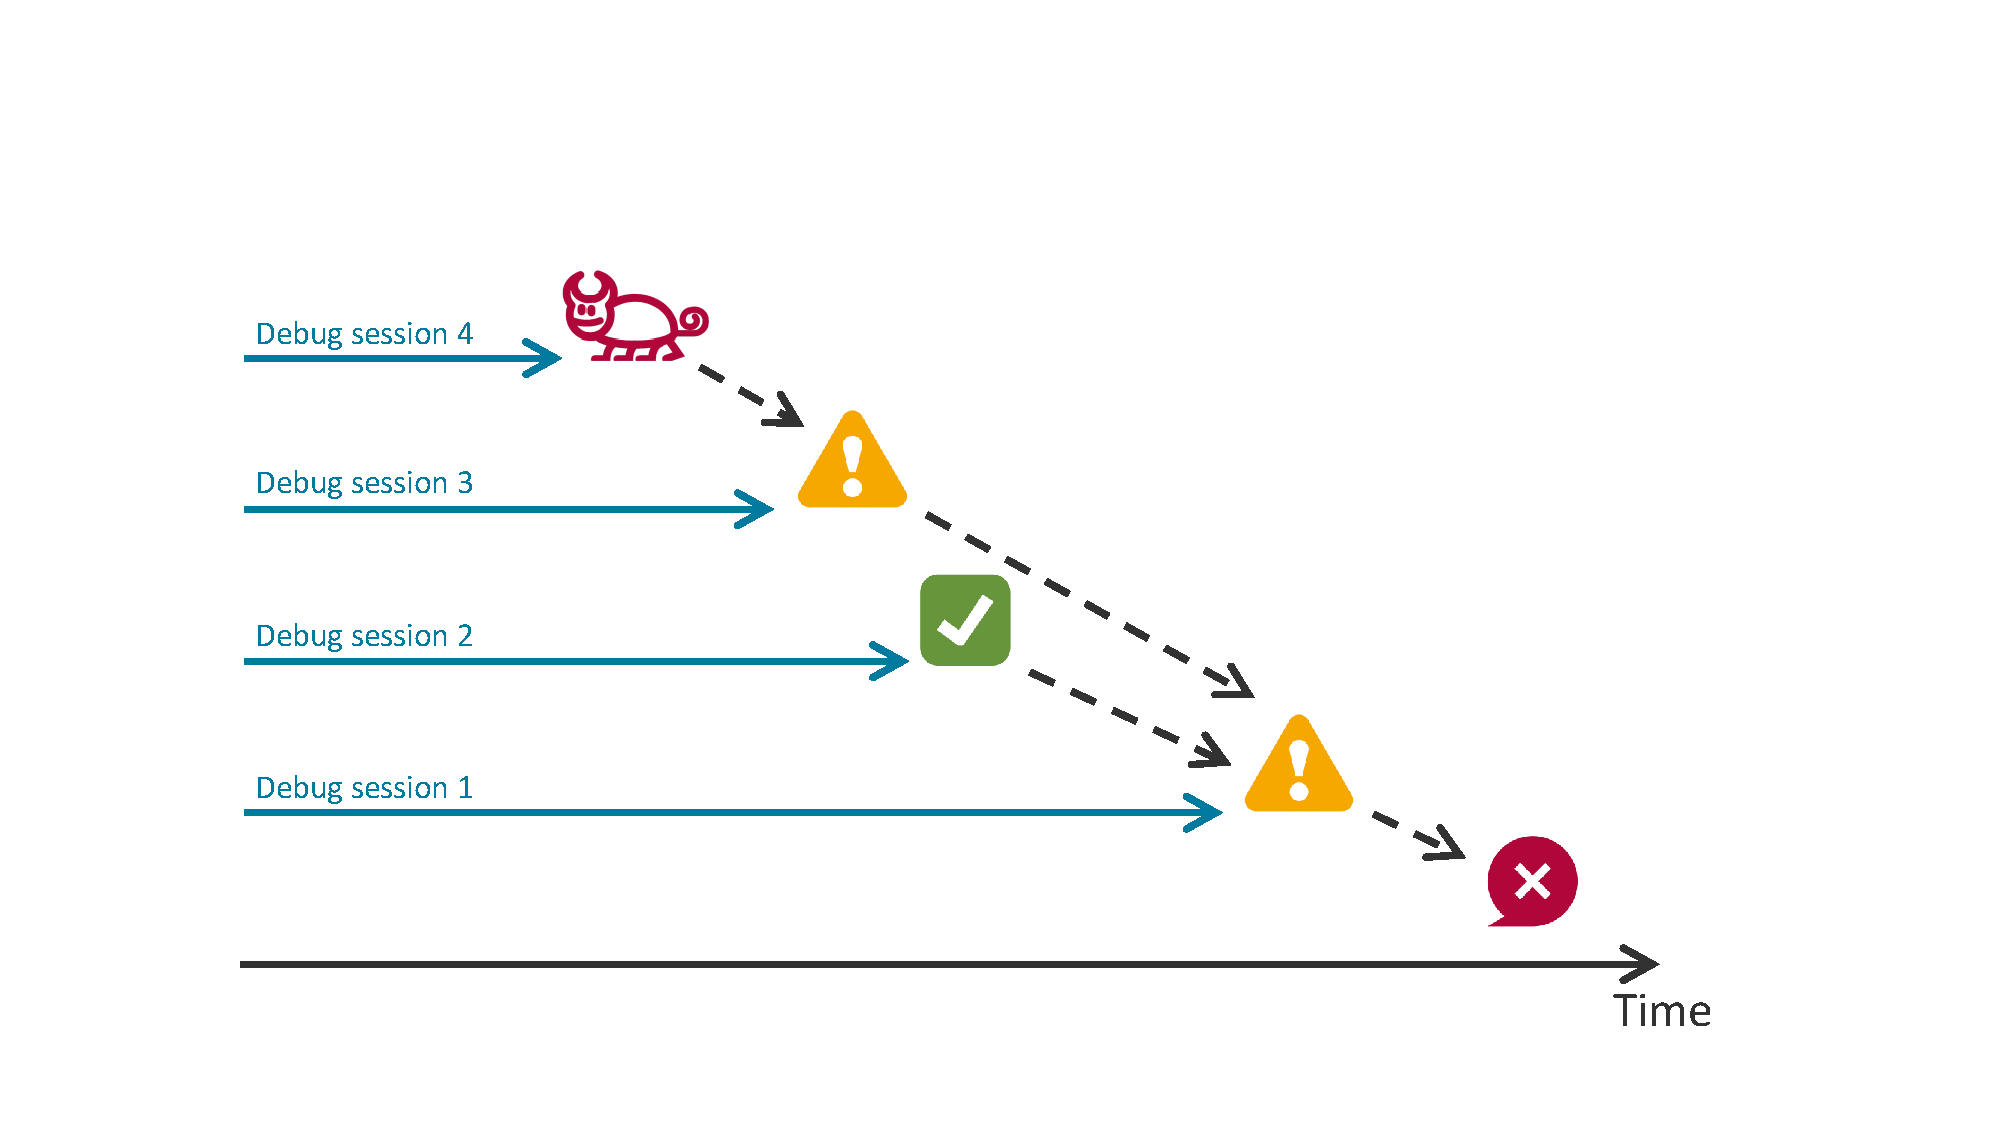
\includegraphics[width=.9\linewidth]{img/workflow-traditional}
\caption{TODO: make a workflow.}
\label{fig:scientifiy-method}
% R. Metzger. Debugging by Thinking - A Multidisciplinary approach.
\end{figure*}
If the experiment does not confirm the hypothesis, developers must improve their understanding of the program in order to form a better one.
If the experiment confirms the hypothesis, however, it has not necessarily revealed the root cause of the failure.
Sometimes, the hypothesis is to vague and the problem needs to be narrowed down further.
In other cases, the experiment revealed that the erroneous behavior of one component was caused by incorrect input of another component, in which case a new failure cause becomes the focus of investigation.
Either way, developers repeat the hypothesis-experiment cycle until they identify the root cause and can begin the repair.

Very often, defective code does not cause the program to fail immediately.
Instead, it creates an error in the program state that propagates, in accordance to the garbage-in-garbage-out principle, until it yields to a failure in a different part of the application.
This sequence of erroneous states is also called the infection chain~\cite{zeller_09_why_programs_fail}.
Developers tasked to locate the defect have to follow the infection chain backwards through execution time.

%Tools can support the fault localization process 

\begin{figure*}[th]
\centering
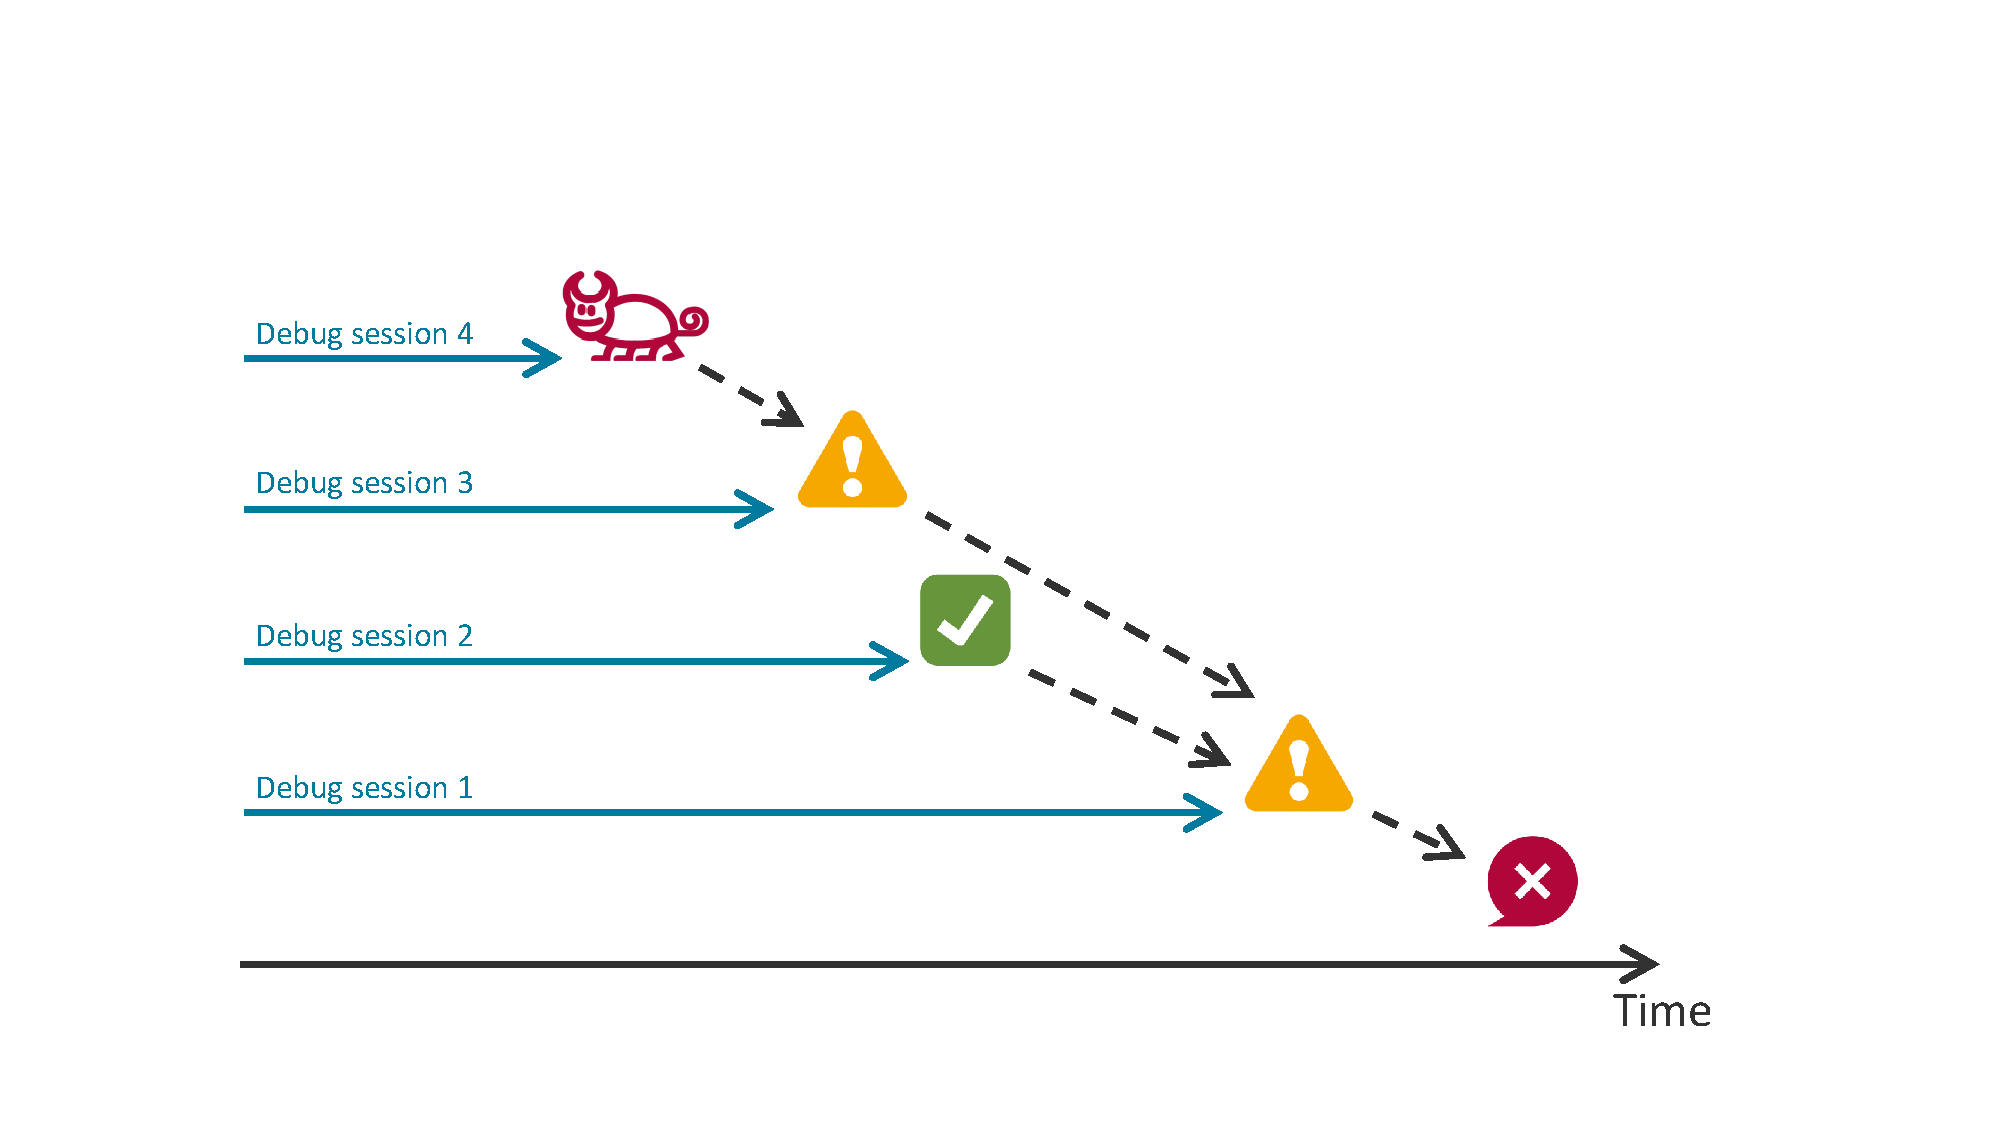
\includegraphics[width=.9\linewidth]{img/workflow-traditional}
\caption{Following an infection chain with a debugger.}
\label{fig:workflow-traditional}
\end{figure*}

\Cref{fig:workflow-traditional} shows how developers track an infection chain with a debugger.
Beginning at the failure, developers follow the infection chain backwards through execution time.
Each step consists of forming a hypothesis and confirming it by inspecting the relevant code location with a debugger.
Following this method, developers will continually get closer to the root cause of the bug.
If developers have not enough knowledge of the program to identify relevant code locations for the next step, the debugger can also be used to explore the program execution to find suspicious locations. 

\section{Advanced Debugging Techniques}

\subsection{Back-in-Time and Omniscient Debugging}

\begin{figure*}[th]
\centering
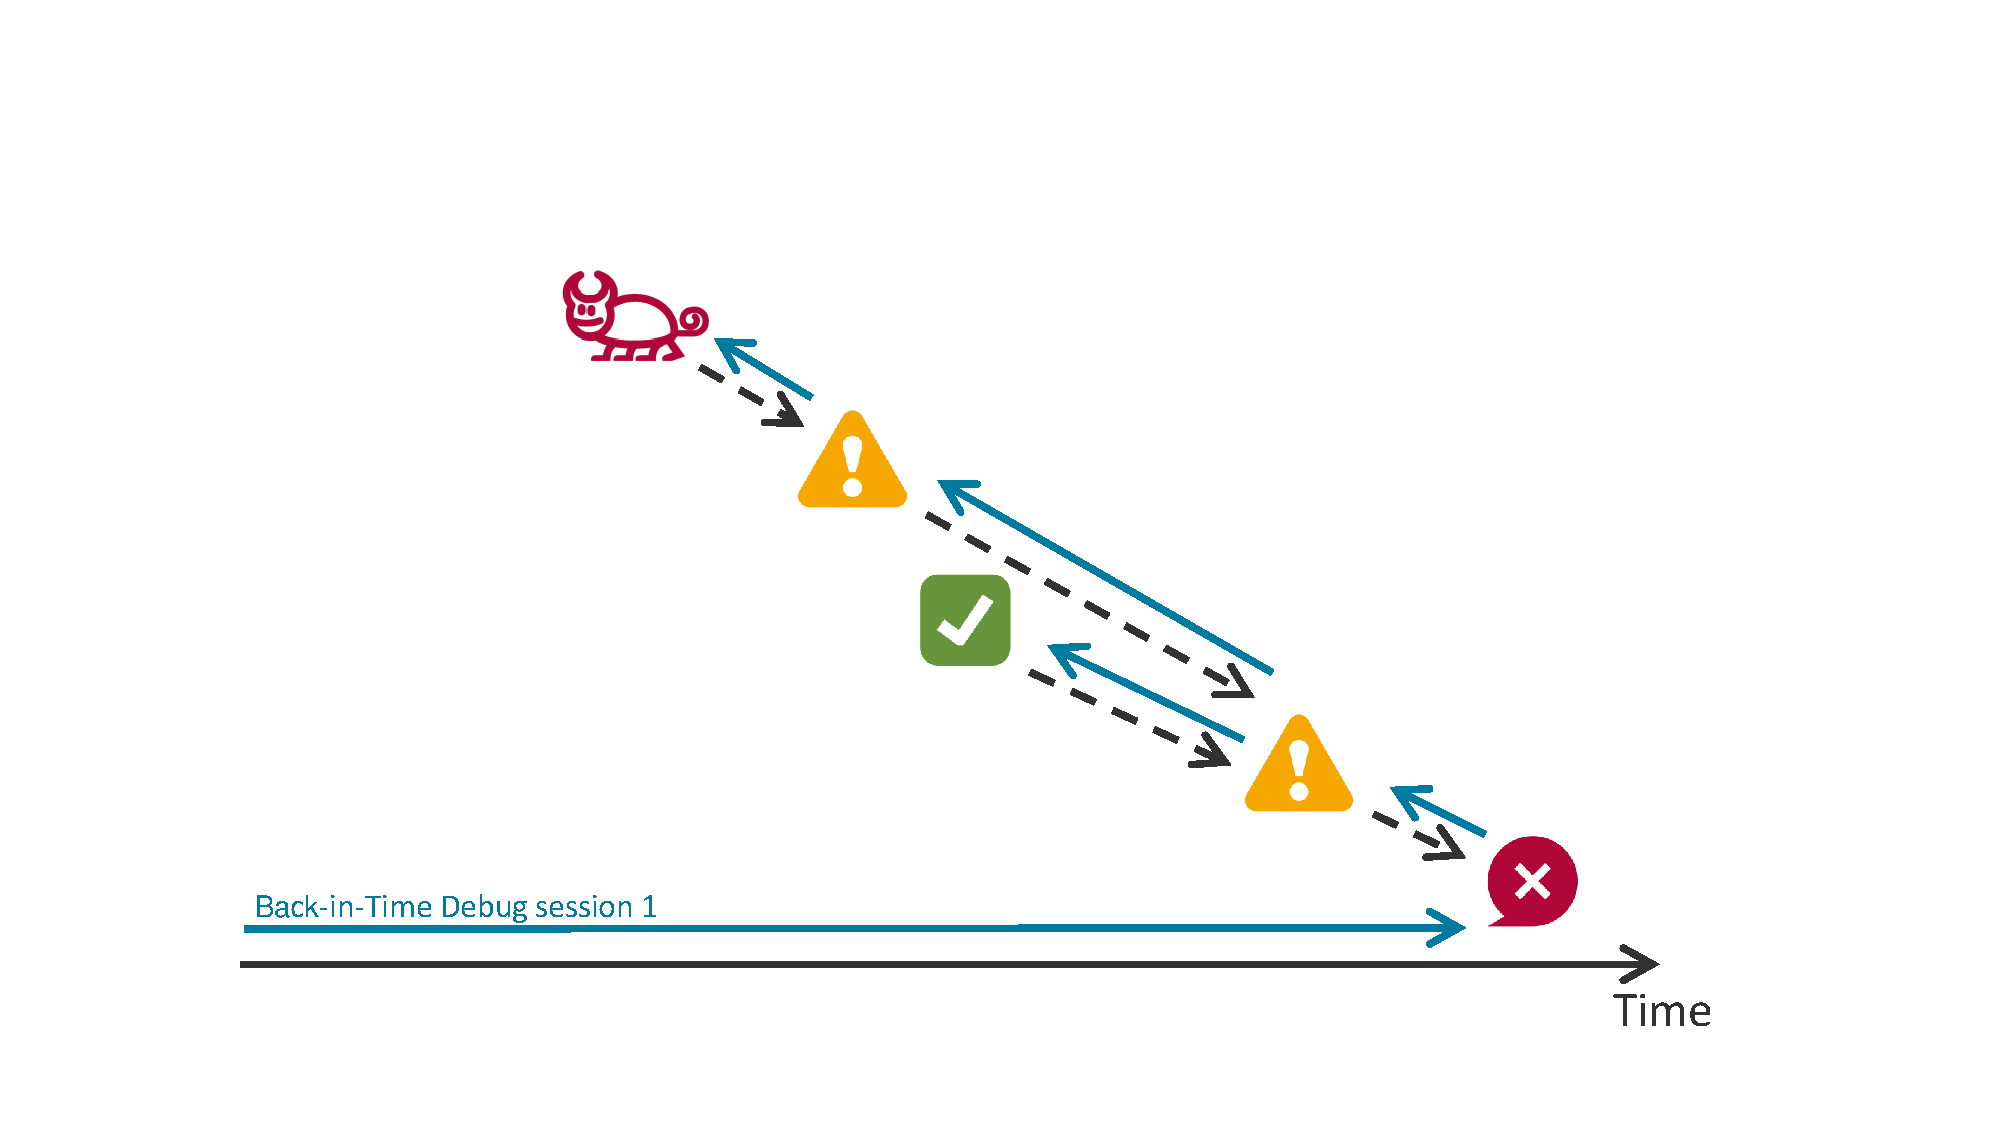
\includegraphics[width=.9\linewidth]{img/workflow-odb}
\caption{Following an infection chain with a back-in-time debugger.}
\label{fig:workflow-odb}
\end{figure*}

%\subsection{Slicing}
\subsection{The Evolution of Slicing Algorithms}

In 1981, Weiser introduced slicing as a technique helping developers to find related code for a given question~\cite{weiser_81_program_slicing}.
According to Weiser, a slice is a subset of a program that, when executed, yields the same state trajectory with respect to given slicing criteria as the original program would have.
The slicing criteria are pairs of variables and code locations.
An important property of the resulting slice is that it must be executable.
This allows the slice to be compiled and inspected with a debugger.

Weiser proposed an algorithm for computing static slices, i.e., slices that are correct for every possible input of the program.
Static slices often are very large, especially for complex applications, and many sophisticated methods have been developed to reduce the size of static slices \todo{ref}.

In 1990, Korel and Laski proposed to compute slices that are valid only for one specific program input~\cite{korel_88_dynamic_program_slicing}.
Such dynamic slices can be much smaller than static slices because the slicer has to consider only one concrete execution path~\cite{venkatesh_95_experimental_results_from_dynamica, hoffner_95_evaluation_and_comparison}.
However, to achieve this we must add the program input to the slicing algorithm's parameters.

Shortly after Korel and Laski, Agrawal and Horgan independently also introduced dynamic slices~\cite{agrawal_90_dynamic_program_slicing}.
Agrawal and Horgan used an approach based on execution traces that allowed to remove more statements than previous approaches, but the resulting slices were not always executable.
Thus, they defined "accurate slices" as slices that contain all statements relevant for computing the state trajectory for the slicing criteria, but are not necessarily compilable or executable.
Agrawal \etal\ also presented SPYDER, a tool that allows debugging non-executable slices by superimposing the slice on an execution of the full program~\cite{agrawal_93_debugging_with_dynamic_slicing}.

Subsequent work focused on increasing the precision of accurate slices, for example in the presence of pointers~\cite{atkinson_02_program_slicing_using_dynamic}.
In 2003, Zhang \etal\ presented three algorithms to efficiently compute "precise slices", i.e., slices that are "accurate" but contain little to no statements that could be removed~\cite{zhang_03_precise_dynamic_slicing_algorithms}.
Like many other authors, Zhang \etal\ argued that producing small slices is essential if slicing is to be "an attractive option" for developers.
However, Korel argued that slicing too aggressively can also be dangerous, as
"for program debugging the challenge is not necessarily to minimize the size of the slice at any cost but rather to minimize the size of the slice without the elimination of faulty program statements"~\cite{korel_98_dynamic_program_slicing_methods}.

The difference between executable and "accurate" slices can be demonstrated with a small example.
In the code shown in \cref{lst:sliceAccurate}, line 9 is only executed during the second iteration of the loop.
Therefore, when choosing ´ratio´ in line 9 as a slicing criterion, "accurate" slicing algorithms can remove the array assignment in line 3.
This will reduce the size of the slice, as the call to ´complexComputation1´ is removed, but when the remaining code is executed, a division by zero will occur during the first iteration in line 7.
Korel argued that the correctness of a slicing algorithm can be objectively determined if it is allowed to produce slices where the program fails.

\begin{lstlisting}[float,caption={Code example for accurate slices.},stepnumber=2,numberfirstline=false,label=lst:sliceAccurate,language=Java]
	void main() {
			float[] data = new float[2];
			data[0] = complexComputation1(); // returns 0.5
			data[1] = complexComputation2(); // returns 5
			for (float f: data) {
					f = adjustValue(f);
					float ratio = 2 / f;
					if (ratio < 1) {
							System.out.println(ratio); // expected 0.2, got 0.4
					}
			}
	}

	float adjustValue(float value) {
			if (false && moreConditions()) { // bug in this line
					return value * 2;
			}
			return value;
	}
\end{lstlisting}

However, algorithms for both executable and "accurate" slices are allowed to remove the call to ´adjustValue´ in line 6 and therefore hide the actual bug.
In general, bugs caused by wrongly skipped or missing code are difficult to locate with slicing.
Wang \etal\ addressed this problem by developing an algorithm to find "relevant" slices, slices including code that could have changed the state trajectory but was not executed~\cite{wang_08_dynamic_slicing_on_java}.
Likewise, Ko \etal\ developed Whyline, a slicing-based tool allowing developers to ask "Why?" and, more importantly, "Why not?" questions~\cite{ko_08_debugging_reinvented_asking}.

By considering developers with a debugging problem as end users of a slicing tool, we can carry the trend of carefully reducing slice sizes to its logical conclusion: we define a "most useful slice" as exactly the subset of statements of a program that developers need to see in order to answer the question they are currently investigating.
Such a slice is not necessarily executable, "accurate", "precise", or "relevant", according to the established definitions, but rather captures the optimal combination of these conflicting properties.

However, to compute a "most useful" slice, we would have to add the developers research question and current state of mind to a slicing algorithm's input.
This leaves us with two problems.
Firstly, we need to find a method to formalize a developer's entire state of mind, and secondly, we need to a way for developers to specify this data easily and correctly.
\todo{Alas, we can not present a solution for either of these problems.
However, as a step towards the goal of "most useful" slices, we developed a slicing algorithm that allows developers to easily get arbitrarily close to the smallest slice they need.}

\section{Additional Challenges in Enterprise Applications}

\tmpStart
To better understand the development of modern business software, we interviewed five software developers from SAP, a German software corporation developing enterprise software to manage business operations.
From these developers, we gained insights on the development of four different projects:
\begin{enumerate}
	\item A software for liquidity risk management that analyzes the cash-flow of financial institutes to assess their liquidity,
	\item A customer analytics software to understand customer behavior based on collected data, which allows, for example, to identify particularly profitable customers or customers that plan to leave the company (e.g., clients of a bank who cancel all their standing orders),
	\item A product for predictive analytics that allows to estimate the probabilities for certain customer behaviors, such as switching distributors or suppliers. The analyses' results are integrated in a customer relationship management (CRM) system and recommend opportunities for salespeople, and
	\item The point-of-sales (POS) explorer, a dashboard that computes various key performance indicators (KPIs) on the revenue and profits of products based on retail data.
\end{enumerate}
%
All applications are designed to work on real-time data generated by respective transactional systems and were developed with an industry partner who provided requirements.

\subsection{Changing Characteristics in 3-tier Applications}

The design of all applications was based on the 3-tier architecture pattern, which divides an application into three layers~\cite{eckerson_95_three_tier_clientserver_architecture}.
The \emph{presentation tier} displays information and receives input from the user,
the \emph{application tier} contains the application's business logic, and
the \emph{data tier} encapsulates data access and persistence.
The presentation tier is the application's front-end and runs on the client, while the application and data tier constitute the back-end and run on the server.

In traditional 3-tier applications, most of the code is implemented in the application layer.
For example, templates allow the application server to render web pages that can be displayed by a browser on the client.
When a dedicated client application is needed, keeping it small and simple reduces the overhead of maintaining and updating a large number of installations.
Either way, the client is little more than a terminal.

On the data side, object-relational mappers (ORMs) allow developers to implement data processing logic directly in the application.
This makes applications independent from specific database products and avoids introducing additional programming languages into the project.
Because application servers can be scaled more easily than databases, this also reduces the database bottleneck that can occur in applications with many users.

Many application frameworks, such as J2EE and Ruby on Rails, follow this philosophy and many tools have been developed to support development and maintenance in such ecosystems.
However, as we found in our interviews, the usefulness of many of such tools is decreasing as technologies and requirements change in the development of modern business applications.

HTML 5 and JavaScript allow to build responsive and dynamic interfaces, which are increasingly expected by users.
Via HTTP and fast connections, megabytes of client code can be updated with every request so there is no longer a need to keep the client code minimal.
JavaScript-based GUI libraries eliminate the need for server-side templates as the entire GUI can be built in the client and data is dynamically loaded via AJAX requests.

With big-data becoming more important for many companies, it is no longer feasible to handle all data operations in the application layer.
Even transactional systems contain a large fraction of analytical operations~\cite{krueger_10_a_case_for_online} and high-performance databases can handle such queries faster than application-level code~\cite{plattner_09_a_common_database_approach}.
Even for transactional operations, the usefulness of ORMs is doubted as they can introduce other organizational and architectural problems~\cite{neward_06_the_vietnam_of_computer}.

All developers reported that their projects followed these new architecture patterns.
To achieve sufficiently low response times, data is stored in \emph{SAP HANA}, a high-performance in-memory relational database.
The application layers run in \emph{SAP HANA Extended Application Services}, an application and web server environment on top of the database.
In each project, the front-end is implement in \emph{SAPUI5}, a JavaScript GUI library based on jQuery.

For the fourth project, the POS explorer, we were given full access to the code base.
At the time of the interview, the whole application had 11 thousand lines of code, libraries excluded.
55\% of the code (i.e., about 6000 lines) was client-side JavaScript, of which about 12\% (725 lines) was data querying code.
The application layer consisted of 2000 lines (18\%) of server-side JavaScript (similar to node.js), while the database layer contained 3000 lines (27\%) of stored procedure code.
Data schema definitions are not included in the line counts, as the data is defined and provided by other applications.
% client/js					2397
% client/fragment		3750
% client/view				 133
% client -- query		 600 // client 6280 -- 6000
% app/xsjs*					2250 //  -- 2000
% db/procedure			2991 // -- 3000
% // 11521

Standards like \emph{OData}~\cite{chappell_11_introducing_odata} allow clients to submit arbitrary queries to the database, entirely eliminating the need for a middle layer.
It should be noted that this setup is different from the classical 2-tier architecture, where a trusted client has full access to the database.
OData still maintains security concerns such as authentication, authorization, and visibility of data, which was previously a responsibility of the application tier.

For one of the projects, the developer reported that they have no application layer code at all.
The application, he estimated, consisted of 90\% client-side JavaScript, of which one-third was OData client code, and 5\% OData service configuration which passed requests to stored procedures that constituted the remaining 5\% of the project.

In conclusion, due to increased complexity of interactions between the different layers it is no longer sufficient to be able to debug each layer on its own.
Instead, tools are needed that help developers to debug and understand the application as a whole.

\subsection{Debugging 3-tier Business Applications}

All developers reported that changes in software development processes affected the way how bugs are handled.
In the past, large applications had separate development teams for front-end, business logic, and data management.
If a team found that a bug was not caused in their respective domain, the responsibility was passed on to the next team.

Agile development methodologies, such as Scrum or Extreme Programming, discourage dividing teams by technology layer.
Instead, requirements and, if necessary, sub-teams are now grouped around feature sets.
Thus, while there still may be developers who are specialized on one of the application tiers, every developer is expected to be able to work on and to debug every layer.
This increases the need for making debugging tools for each layer easily available to all developers.

The existence of bugs is typically discovered by observing unexpected data in the user interface.
Then, developers use their browser's development tools to examine the request with which the data was obtained.
In most cases, the response data is passed unchanged to the GUI components and the incorrect data can be tracked directly back to the response.
Here, the first uncertainties occur as it is often not obvious whether the request was submitted with incorrect arguments or whether the error is on the server-side.

If developers decide to continue to the application code, they determine which server function is called, connect a debugger to the application server, set a breakpoint, and re-submit the failing request.
Then they use the debugger to understand how the request is processed.

If no fault can be found, they now need to determine if the results returned by database queries are correct.
For queries that include complex views or stored procedures, this is not an easy task.
Furthermore, if the query was composed at runtime, developers also need to determine the actual query string and which arguments were used.
After that, they can use the tools provided by the database client to analyze the query and verify the result.

Using these methods, developers move up and down the stack until they find the root cause of the bug.
Generally, all developers reported that they preferred to work with a top-down approach, i.e., they try to first understand the interaction between the layers before starting a debugger to narrow down possible locations for the bug as early as possible.
However, while the developer tools of browsers were reported to be somewhat useful for this task, no such tools exist to understand the interaction between application and data tier at a glance.

Overall, frequent switches between tools were reported to be a major distraction when trying to focus on the program flow.
Often, multiple monitors were used to allow developers to access all tools more quickly, but all developers wished for better integration between tools.
\tmpEnd

\section{Requirements}

Requirements
- Iterative approach
- Identify related statements
- support short-term memory
- reduce problem size

%Finding bugs in complex code is a demanding task for developers and many tools and techniques have been developed to support this process.
%However, complex system architectures add another level of difficulty to fault localization.
%
%Server-based applications typically use a three-tier architecture.
%The database layer is used to persist the application's domain model.
%The user interface layer shows application data to the user and accepts user input.
%In between, the application layer contains most of the business logic which defines the application's workflows, how to handle user requests, and how to collect and present requested data.
%
%When most code resides in the application layer, so do most bugs and the well-known debugging tools can be used to locate them.
%However, in more recent years, the classic three-tier architecture changed in multiple ways.\todo{source}
%
%\subsection{Database Layer}
%
%The amounts of data to be handled by server-based applications are always increasing.
%Recently, big data has become a very important topic for many enterprises.
%To guarantee optimal performance on large data sets, more and more data handling code has to move closer to data, into the database layer.\todo{source}
%
%tbd: describe UI technologies
%
%\subsection{User-Interface Layer}
%
%Better web browsers, HTML 5, and Java Script replaced the terminal application.
%It is now easier to manage client code as updates are automatically requested via HTTP.
%This way, more business logic could move into the UI layer to provide a better user experience.\todo{source}
%
%tbd: describe UI technologies
%
%\subsection{Application Layer}
%
%Remaining AppLayer: request mapping, security
%
%Java, Rails, Node.js
%
%skip applayer with ODATA and user-management in database
%
%\subsection{Debugging the Stack}
%
%Both modern browsers and databases have debugging capabilities that are useful to locate bugs within their respective layers.
%Alas, not every bug can be tracked down to a single code location. 
%Sometimes, it is a combination of mismatching assumptions in different code locations that compose the fault \todo{source}.
%In a complex system, these locations need not reside in a single component, but can be scattered across all layers.
%Likewise, the infection chain that connects the observed failure with the fault in the code can cross several system boundaries.
%
%In both cases, no single debugging tool is sufficient to locate the bug, as each debugger can only be used to debug its respective system.
%The resulting tool and context switches impose a mental overhead that distracts developers from the actual problem.
%
%The problem is further amplified with service-oriented architecture (SOA), and micro-services in particular.
%To achieve better scalability and faster life-cycle management, applications are broken down into many independent systems, each with their own database.
%While the resulting modularization can help to limit the consequences of software failures to smaller sub-systems, the difficulty of locating cross-system bugs increases further.
%
%%The debugger is one of the most important tools of a software developer. 
%%It allows to observe and inspect a program’s execution and can be used for many purposes, such as bug detection and code comprehension. 
%%Workflow
%%\\- failure observed
%%\\- error in state- > find the code
%%\\- either GIGO, then repeat, or...
%%\\- fault in code
